\section{Harmonic Oscillator - 谐振}
Suppose a degree of freedom $x$ (position, angle, current, stress, etc.) is subject to some potential function $V(x)$. We wish to zoom-in and ask what is the effective potential for this degree of freedom close to a stable equilibrium of the potential (local minimum). \\
We assume near $x_0$, we may Taylor expand the potential function to be:
$$V(x) = V(x_0) + V'(x_0)(x - x_0) + \frac{1}{2}V''(x_0)(x-x_0)^2 + \dots$$
Since we are analyzing near a local minimum, we have $V'(x_0) = 0$ and $V''(x_0) > 0$. By ``ignoring'' the smaller terms, we essentially have:
$$V(x) \approx V_0 + \frac{1}{2}V''(x_0)(x-x_0)^2$$
which is a quadratic potential, or a harmonic potential.

\subsection{Classial Harmonic Oscillator - 经典谐振}
A classical harmonic oscillator has the equation of motion:
$$m \cdot \pdv[2]{t} x = -\pdv{V}{x} = -V''(x_0)(x-x_0)$$
This solution to this differential equation is
$$x(t) = A \cos(\omega(t - t_0)) + x_0, \omega = \sqrt{\frac{V''(x_0)}{m}}$$
Some classical examples are springs, the pendulum, molecular vibration, fluctuating fields, LC circuits, and phonons in lattice.

\subsection{Quantum Harmonic Oscillator - 量子谐振}
For a quantum harmonic oscillator, the Hamiltonian is:
$$\hamiltonian = \frac{\opmtm^2}{2\mu} + \frac{1}{2}\mu \omega^2 \oppos^2$$
where we set $V_0 = 0$, $x_0 = 0$, it being time-independent, and we are working in a 1D continuous space. \par
Our goal here is to solve the Schr\"odinger's Equation for $\hamiltonian$, which is by solving the eigenvalue problem $\hamiltonian \ket{n} = E_n \ket{n}$, and find all the stationary states. \par
The Schr\"odinger's Equation is as follows:
$$-\frac{\hbar^2}{2\mu} \pdv[2]{x}\psi_n(x) + \frac{1}{2}\omega^2 x^2 \psi_n(x) = E_n \psi_n(x)$$
This equation can be solved analytically by directly diagonalize $\hamiltonian$, which is an algebraic approach, instead of a direct solution. \par
We start by defining some ``ladder'' operators:
\begin{definition}
    The \uimpt{annihilation operator} is defined to be:
    $$\annih = \sqrt{\frac{\mu \omega}{2\hbar}}\oppos + \imag \frac{1}{\sqrt{2\mu\omega\hbar}}\opmtm$$
    The corresponding \uimpt{creation operator} is the complex adjoint of the annihilation operator, which is:
    $$\creat = \sqrt{\frac{\mu \omega}{2\hbar}}\oppos - \imag \frac{1}{\sqrt{2\mu\omega\hbar}}\opmtm$$
\end{definition}
This means, the position observable and the momentum observable can be expressed in terms of these operators in the following way:
\begin{align*}
    \oppos &= \sqrt{\frac{\hbar}{2\mu\omega}}(\annih + \creat) \\
    \opmtm &= -\imag \sqrt{\frac{\mu \omega \hbar}{2}}(\annih - \creat)
\end{align*}
By utilizing $[\oppos, \opmtm] = \imag \hbar \id$, we have
\begin{lemma}
    The commutator of the annihilation and creation operator is:
    $$[\annih, \creat] = \id$$
\end{lemma}
This lemma can be shown by directly commuting the two operators with the position-momentum commutator being used in the process. \par
By defining such operators, we can then express the Hamiltonian with them, and through substituing $\oppos, \opmtm$ in terms of $\annih, \creat$, we have:
$$\hamiltonian = \hbar \omega (\creat \annih + \frac{1}{2}\id)$$
\begin{definition}
    Define the \uimpt{number operator} $\hat{n}$ to be:
    $$\hat{n} = \creat\annih$$
\end{definition}
It is trivial to see that $[\hamiltonian, \opnum] = 0$, and $\opnum$ is \impt{Hermitian}. That means, it is a conserved quantity for $\hamiltonian$, and if we solve the eigenvalue problem for $\opnum$, we solve the Schr\"odinger's Equation. \par
Let $\ket{n}$ be the eigenvector of $\opnum$, then $\opnum \ket{n} = n \ket{n}$, and so far $n$ is open and unknown. Then, from $[\opnum, \creat] = \creat$ and $[\opnum, \annih] = -\annih$, we have:
\begin{align*}
    \opnum(\creat\ket{n}) &= \creat(\opnum\ket{n}) + \creat\ket{n} \\
    &= \creat(n\ket{n}) + \creat\ket{n} \\
    &= (n+1) \creat\ket{n} \\
    \opnum(\annih\ket{n}) &= (n-1)\annih\ket{n}
\end{align*}
So, $\creat\ket{n}$ is an eigenvector of $\opnum$ with eigenvalue $n+1$; $\annih\ket{n}$ is an eigenvector of $\opnum$ with eigenvalue $n-1$. Since $\opnum$ has a non-degenerate eigenspace, we have $\creat\ket{n} \propto \ket{n+1}$ and $\annih \ket{n} \propto \ket{n-1}$. Assume that $\ket{n}$ are normalized, that is $\braket{n} = 1$ (restricting mathematical solutions to physical solutions), when we define:
$$\ket{\tilde{n+1}} = \creat \ket{n}$$
We have the $\braket{\tilde{n+1}} = n + 1$. By applying the same logic to $\creat \ket{n}$, we have two important properties:
\begin{align*}
    \creat \ket{n} &= \sqrt{n+1}\ket{n+1} \\
    \annih \ket{n} &= \sqrt{n} \ket{n-1}
\end{align*}
We first know:
$$\forall v \in \hilbert, \mel{v}{\opnum}{v} = \mel{v}{\creat\annih}{v} = \braket{av}{av} \ge 0$$
This means $n$ must be non-negative real numbers, as $\ket{n}$ are also part of the Hilbert space. \\
Next, let $k$ be a non-negative integer, we have
$$0 \le \mel{n}{\opnum^k}{n} = \mel{n}{(\creat)^k(\annih)^k}{n}$$
This further derives to:
\begin{align*}
    \mel{n}{(\creat)^k(\annih)^k}{n} &= \mel{n-1}{(\creat)^{k-1}(\annih)^{k-1}}{n-1} \cdot \sqrt{n} \cdot \sqrt{n} \\
    &= \braket{n-k} \cdot n \cdot (n-1) \cdot \dots \cdot (n-k+1)
\end{align*}
This means, $n$ must be a non-negative integer, otherwise, there exists a $k$ such that the series product will be negative. \par
We find for the Hamiltonian $\hamiltonian = \hbar \omega (\creat \annih + \frac{1}{2}\id)$ has eigenvalues $\{\frac{1}{2}\hbar\omega, \frac{3}{2}\hbar\omega, \frac{5}{2}\hbar\omega, \dots\}$ for normalizable eigenvectors. \\
Now we need to construct the corresponding eigenstates. We first start with $\ket{0}$, we know $\annih \ket{n} = \sqrt{n}\ket{n-1}$, so $\annih\ket{0} = \vec{0}$. The annihilation operator on the position wavefunction is:
$$\annih: \psi(x) \mapsto \sqrt{\frac{\mu \omega}{2\hbar}} \cdot x \cdot \psi(x) + \imag \frac{1}{\sqrt{2\hbar \mu \omega}} (-\imag \hbar)\pdv{x}\psi(x)$$
Therefore, the differential equation for $\psi_0(x)$ (the position wavefunction of $\ket{0}$) is:
\begin{align*}
    \frac{1}{\sqrt{2\hbar}}(\sqrt{\mu\omega}x + \frac{\hbar}{\sqrt{\mu\omega}}\pdv{x})\psi_0(x) &= 0 \\
    \psi_0(x) &= \frac{1}{\sqrt[4]{\frac{\hbar\pi}{\mu\omega}}} \cdot \exp(-x^2 \cdot \frac{\mu\omega}{2\hbar})
\end{align*}
For other $n \in \N$, we start with $\creat\ket{n} = \sqrt{n+1}\ket{n+1}$, then this gives:
$$\creat\ket{0} = \sqrt{n!}\ket{n}$$
which means the position wavefunction of $\ket{n}$ is essentially:
$$\psi_n(x) = \frac{1}{\sqrt{n!}} (\creat)^n \psi_0(x) = \frac{1}{\sqrt{n!}} (\sqrt{\frac{\mu\omega}{2\hbar}}x - \imag \frac{-\imag \hbar}{\sqrt{2\hbar\mu\omega}}\pdv{x})^n \psi_0(x)$$
This eventually solves to:
$$\psi_n(x) = \frac{1}{n! \cdot (\frac{2\hbar}{\mu\omega})^n\sqrt{\frac{\hbar\pi}{\mu\omega}}} \cdot H_n(x) \cdot \exp(-x^2 \cdot \frac{\mu\omega}{2\hbar})$$
where $H_n(x)$ are the \impt{Hermite polynomials}.
\begin{center}
    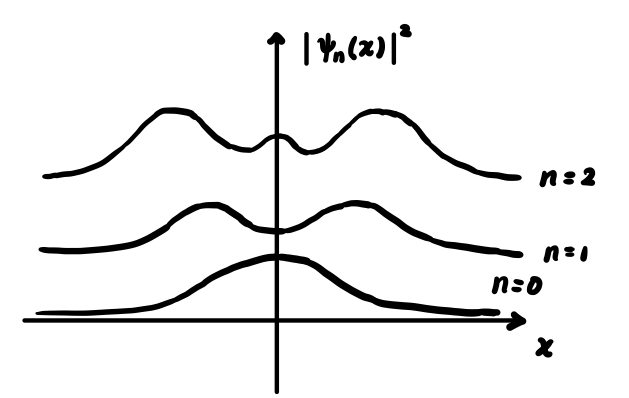
\includegraphics[scale = 1]{ho-prob-dist.png}
\end{center}
Note that the normalizability condition for $\ket{n}$ led to a discrete energy spectrum. The minimal energy $E_0 = \frac{1}{2}\hbar\omega$, meaning that the harmonic oscillator is never at rest, this is the ``zero-point'' energy. \\
It is also possible to discuss the ``classical limits''. This is considering the high energy eigenstates where $n$ is much larger than $1$. It thus has the probability distribution of:
\begin{center}
    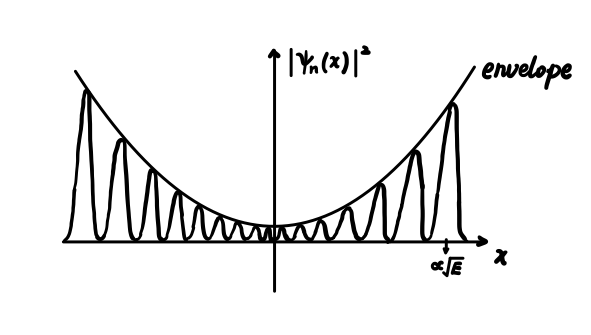
\includegraphics[scale = 1]{ho-high-energy.png}
\end{center}
The probability distribution approaches the classical probability distribution emerged over time, up to fluctuations, $n$ is the number of fluctuations. This ``envelope'' is the probability distribution in $x$ averaged over time. \\
Take a pendulum as an example, where the $x$ of interest is the angle. If we look at the angle at random times, the time-averaged ``angle'' will have an angle density for angle $p(x)$. The pendulum stays longer at the maximum height, and stays shorter at the minimum height. 
\begin{center}
    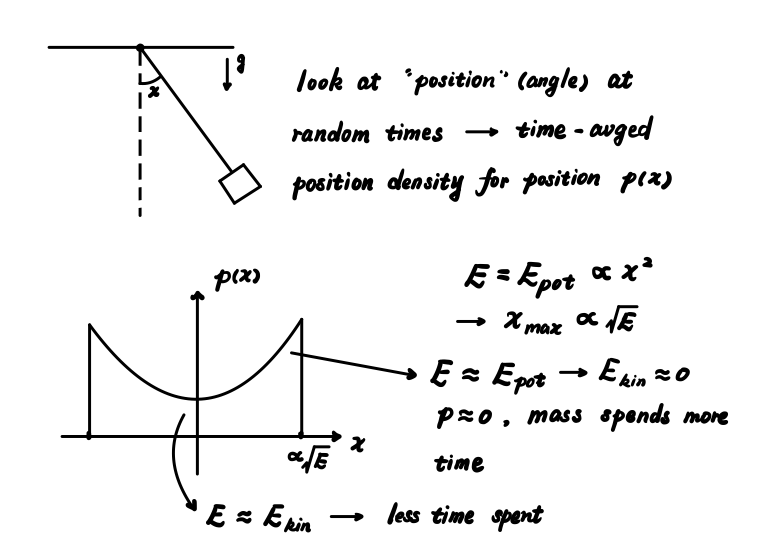
\includegraphics[scale = 1]{ho-classical-lim.png}
\end{center}
Be careful that the energy eigenstates are stationary, so $\expval{\oppos}_t, \expval{\opmtm}_t$ remains constant, there is no oscillations observable from these two observables.
\begin{definition}
    \uimpt{Coherent states} are classically oscillating quantum states, typically denoted by $\ket{\alpha}, \alpha \in \C$
\end{definition}
If we plot the position observable and momentum observable expectation values, we have:
\begin{center}
    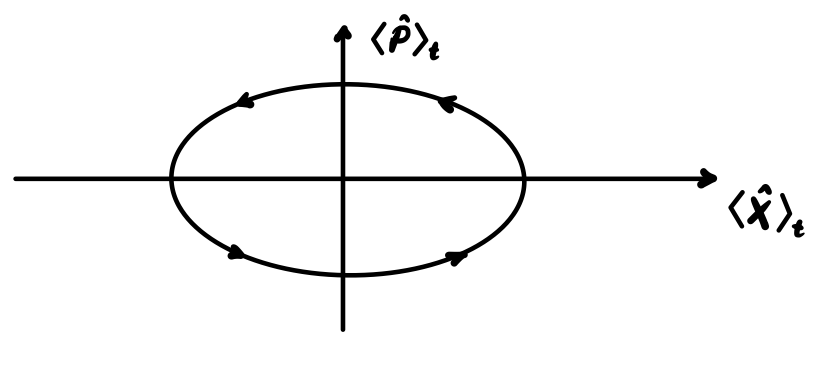
\includegraphics[scale = 1]{coherent-state.png}
\end{center}
It is going to oscillate around with uniform velocity in the ellipse, and we can map the $x$-component to $\sin$ and the $y$-component to $\cos$. A laser field can be such an example.

\newpage